\begin{tikzpicture}

\GraphInit[vstyle=Classic]

\Vertex[Lpos=-90,x=10, y=0, L=$p_{1}$]{p1};
\Vertex[Lpos=-90,x=8, y=0, L=$p_{2}$]{p2};
\Vertex[Lpos=-90,x=6, y=0, L=$p_{s - 3}$]{psm3};
\Vertex[Lpos=-90,x=4, y=0, L=$p_{s - 2}$]{psm2};
\Vertex[Lpos=-90,x=2, y=0, L=$p_{s - 1}$]{psm1};
\Vertex[Lpos=-90,x=0, y=0, L=$p_{s}$]{ps};

\Edge[style ={-},label={$a_{2}$},labelstyle={above}]({p1})({p2})
\Edge[style ={draw=none},label={$(a_{1})$},labelstyle={below}]({p1})({p2})
\Edge[style ={-, dashed}]({p2})({psm3})
\Edge[style ={-},label={$a_{s - 2}$},labelstyle={above}]({psm3})({psm2})
\Edge[style ={draw=none},label={$(a_{s - 3})$},labelstyle={below}]({psm3})({psm2})
\Edge[style ={-},label={$a_{s - 1}$},labelstyle={above}]({psm2})({psm1})
\Edge[style ={draw=none},label={$(a_{s - 2})$},labelstyle={below}]({psm2})({psm1})
\Edge[style ={-},label={$a_{s}$},labelstyle={above}]({psm1})({ps})
\Edge[style ={draw=none},label={$(a_{s - 1})$},labelstyle={below}]({psm1})({ps})

\end{tikzpicture}
